\chapter{\IfLanguageName{dutch}{Stand van zaken}{State of the art}}%
\label{ch:stand-van-zaken}

% Tip: Begin elk hoofdstuk met een paragraaf inleiding die beschrijft hoe
% dit hoofdstuk past binnen het geheel van de bachelorproef. Geef in het
% bijzonder aan wat de link is met het vorige en volgende hoofdstuk.

% Pas na deze inleidende paragraaf komt de eerste sectiehoofding.

\section{Inleiding}
Welkom bij het onderdeel 'stand van zaken'. 
Dit onderdeel omvat een uitgebreide literatuurstudie waarin enkele topics behandeld worden die relevant zijn met de probleemstelling die eerder geschetst werd. 
Het is verdeeld in verschillende onderdelen: de eerste drie zullen een probleem beschrijven dat enerzijds geobserveerd werd door professionals op de 
werkvloer en anderzijds geconstateerd werd door mee te kijken over de schouder van een van die professionals en zodoende hun workflow te observeren en te ontleden. 

De volgende drie onderdelen zullen handelen over mogelijke obstakels en belangrijke principes die men in het achterhoofd moet houden wanneer men een tool ontwikkelt die beantwoordt aan de probleemstelling.\\ 

Ook wordt kennis gemaakt met verschillende technische aspecten (zoals \Gls{LLM}'s) die fundamentele bouwstenen vormen voor een dergelijke implementatie. 
De kennis die hier door de lezer verworven wordt is essentieel om de verdere hoofdstukken comfortabel door te kunnen nemen en te begrijpen. 

Het laatste onderdeel handelt over de structuur en werking van het Technology Acceptance Model. 
Hier wordt onderbouwd hoe efficiënt het kan zijn en hoe een ontwikkelaar er het meest efficiënt gebruik van kan maken.

\newpage


\section{Inefficiënt documentmanagement en repetitie}
In een advocatenkantoor is het vanzelfsprekend dat er op dagelijkse basis heel veel documenten aangemaakt en verwerkt worden.
Denk maar aan het opstellen van dagvaardingen, ingebrekestellingen, e-mails, aangetekende brieven en andere communicatie.

Natuurlijk dringt zich dit op dat deze taken veel tijd in beslag kunnen nemen. Naast een administratief spectrum gaat het ook over verdediging van cliënten, pleiten en ander rechtbankwerk.

Een groot deel van het opstellen van documenten in een advocatenkantoor is werk dat heel repetitief in aard is. 
Denk maar aan manueel opzoekwerk, copy-pasten van informatie, ... 
Dit werk valt onder een workflow die in aanmerking komt voor automatisatie. 
De manuele uitvoering ervan kan ervoor zorgen dat het frustrerend wordt voor een advocaat om uit te voeren. \\

Repetitief werk is ook zeker geen probleem dat zich beperkt binnen de advocatuur. 
Als we kijken naar waar een gemiddelde kantoormedewerker zoal tijd aan spendeert, zien we dat ze 10\% van hun tijd spenderen aan het manueel invoeren van data in businessapplicaties(zoals \Gls{ERP} of \Gls{CRM} programma's). 
Ook kunnen we zien dat 50\% van hun tijd gaat naar het maken en updaten van documenten zoals PDF's, spreadsheets of tekstdocumenten. \autocite{Workfellow} \\ 

Natuurlijk zijn advocaten niet 100\% van hun totale werktijd op kantoor. 
De makkelijk te automatiseren aard van sommige van bovenstaande taken kan er dus voor zorgen dat een advocaat kostbare tijd bespaart, dus is het heel zinvol om toch een deel ervan te automatiseren. 
Er kan hier frustratie ontspringen uit de combinatie van de taken niet graag uitvoeren en het feit dat ze waarschijnlijk makkelijk te automatiseren zijn. \\

Het feit dat deze taken zo lang duren kan gewijd worden aan verschillende zaken: men investeert te weinig tijd in efficiëntie(zoals sneltoetsen leren kennen, efficiënte templates en stijlen maken, ...), 
men heeft geen tijd om automatisatie eigenhandig aan te pakken (scripttalen leren schrijven, aankoop van software, ...), enzoverder. 

In deze bachelorproef nemen we de tijd om te onderzoeken welke tools en technologieën er te pas komen bij de automatisatie van bepaalde taken. 
We zullen beginnen bij het begin, hoe ontstaat repetitie? En nog belangrijker, hoe kunnen we het wegwerken? 

Repetitie is een algemeen gekend probleem dat kan ontstaan door verschillende oorzaken, 
zoals een te groot (of ongeorganiseerd) archief van documenten of verschillende obstakels en valkuilen tijdens het opzoeken en verwerken van informatie. 

\newpage


\section{Het managen van grote hoeveelheden documenten}
\subsection{Probleemstelling}
Doorheen de jaren wordt er een heel groot archief aan documenten opgebouwd, denk maar aan communicatie, dossiers, facturen enz.
Het doorzoeken en onderhouden van dergelijk archief kan enerzijds heel complex worden en anderzijds onnodig veel tijd in beslag nemen.
Zodoende kan de productiviteit van een kantoor in het nauw gedreven worden.

Hoe (her)organiseer je zo een archief? Hoe kan je er het best in zoeken? Hoe kan er tijd bespaard worden?

\subsection{Mogelijke hulpmiddelen en oplossingen}
In eerste instantie is het opzoeken in een archief belangrijker op korte termijn dan een volledige herstructurering. Een archief is al lang niet meer een oude metalen kast die in de kelder van een
kantoor staat. Dit is bij de meeste bedrijven al lang geëveolueerd naar een digitale dataset. Moet deze dan constant manueel doorzocht worden?

Het opzoeken van documenten in een digitaal archief is een mooi voorbeeld om te vergelijken tussen menselijke en machinale zoekmethodes.
Het kan immers parallel gesteld worden met een online zoekmachine. Volgende citatie geeft ons een korte introductie over zoekmachines.

\begin{displayquote}
	\textit{"Search engines have been with us for several decades as an integral part of our digital life.
		We are casually searching over billions of web pages to retrieve and share information from various resources.
		While humans are very good at conversational context and background knowledge which helps them to deal with intrinsic ambiguity of words,
		it may not be true in case of search engines."} \autocite{MediumSemanticSearch}
\end{displayquote}

Het artikel gaat dan verder en zegt dat er iets bestaat als 'Semantisch zoeken'. Semantisch zoeken zal niet alleen naar de letterlijk ingevoerde woorden van een zoekterm kijken,
maar zal ook de betekenis, context en het algemeen onderwerp er uit proberen extraheren. Dit helpt om relevante resultaten te bieden en kan bereikt worden via Natural Language Processing, oftewel NLP.

Zoekmachines, en zeker degene uit de "primitieve" generatie, gebruikten echter niet altijd een semantische methodiek:

\begin{displayquote}
	\textit{"At first, search engines were lexical: the search engine looked for literal matches of the query words,
		without understanding of the query’s meaning and only returning links that contained the exact query."} \autocite{MediumSemanticSearch}
\end{displayquote}

Lexicaal zoeken is (relatief gezien) simpel te implementeren, dus een "primitief" concept dat letterlijke matches zoekt van de query in een bepaalde dataset.
Semantisch zoeken is daarentegen wat complexer in opbouw.

\begin{displayquote}
	\textit{"On the other hand, “Semantic Search” can simplify query building, because it is supported by automated natural language processing programs
		i.e. using Latent Semantic Indexing — a concept that search engines use to discover how a keyword and content work together to mean the same thing."} \autocite{MediumSemanticSearch}
\end{displayquote}

Semantisch zoeken is hier vooral een toepasbare topic omdat het erg afhankelijk is van NLP, een van de belangrijkste topics van deze paper.

Nu, een zoekmachine is dus een polyvalente tool, die kan worden ingezet op verschillende, variërende datasets.
Dit kan dus bijvoorbeeld een volledig archief zijn van documenten in een advocatenkantoor.
Het implementeren van een semantisch zoekalgoritme kan een oplossing bieden op het inefficiënt zoeken in dit archief.

Waarom zouden we hier geen lexicaal zoekalgoritme toepassen?
Omdat contextueel zoeken is soms iets heel belangrijk kan zijn, het kan perfect zijn dat men zoekt voor iets dat niet letterlijk (alle) zoektermen kan bevatten.

Een lexicaal algoritme is dus niet de beste oplossing omdat het tekort kan schieten in bepaalde gevallen. Medium illustreert dit ook aan de hand van LSI:

\begin{displayquote}
	\textit{"In brief, LSI(Latent Semantic Index) does not require an exact match to return useful results.
		Where a plain keyword search will fail if there is no exact match,
		LSI will often return relevant documents that don’t contain the keyword at all." }\autocite{MediumSemanticSearch}
\end{displayquote}

\section{Obstakels in research van rechtszaken}
\subsection{Probleemstelling}
Bij een (oppervlakkige) verkennende audit bij advocatenkantoor Deltalex viel op dat er veel tijd wordt gespendeerd aan het opzoeken van dossiergerelateerde informatie.
Denk hierbij maar aan contactgegevens (ondernemingsnummer, adres, ...) van een cliënt, dossierdata, technische specificaties, enz.
In het vorige deel werd al besproken dat zoekmachines ons hiermee kunnen helpen. Deze kunnen documenten teruggeven die een goeie match zijn met onze zoekcriteria.
Maar hoe giet dit met in een antwoord van bv. een digitale assistent?

\subsection{Mogelijke hulpmiddelen en oplossingen}
Voor een advocaat kan het formuleren van een antwoord (gebaseerd op een zoekresultaat) een lang en repetitief proces vormen indien manueel uitgevoerd.
Gelukkig kunnen hier technieken zoals RAG (Retrieval-Augmented Generation) een grote hulp bij bewijzen.

RAG (Retrieval Augmented Generation) is een van de grootste use cases voor LLM's(Large Language Models) en is een framework dat de fundamentele trainingsdata van een Large Language Model
combineert met bestaande data in een database. Zodoende kan een model gegronde antwoorden geven, gebaseerd op betrouwbare en relevante informatie.

Een quote van Medium legt uit hoe RAG werkt in grote lijnen:

\begin{displayquote}
	\textit{"A typical RAG process, as pictured below, has an LLM, a collection of enterprise documents, and supporting infrastructure to improve information retrieval and answer construction.
		The RAG pipeline looks at the database for concepts and data that seem similar to the question being asked, extracts the data from a vector database and reformulates the data into
		an answer that is tailored to the question asked. This makes RAG a powerful tool for companies looking to harness their existing data repositories for enhanced decision-making
		and information access."} \autocite{MediumRAG}
	\begin{figure}[h]
		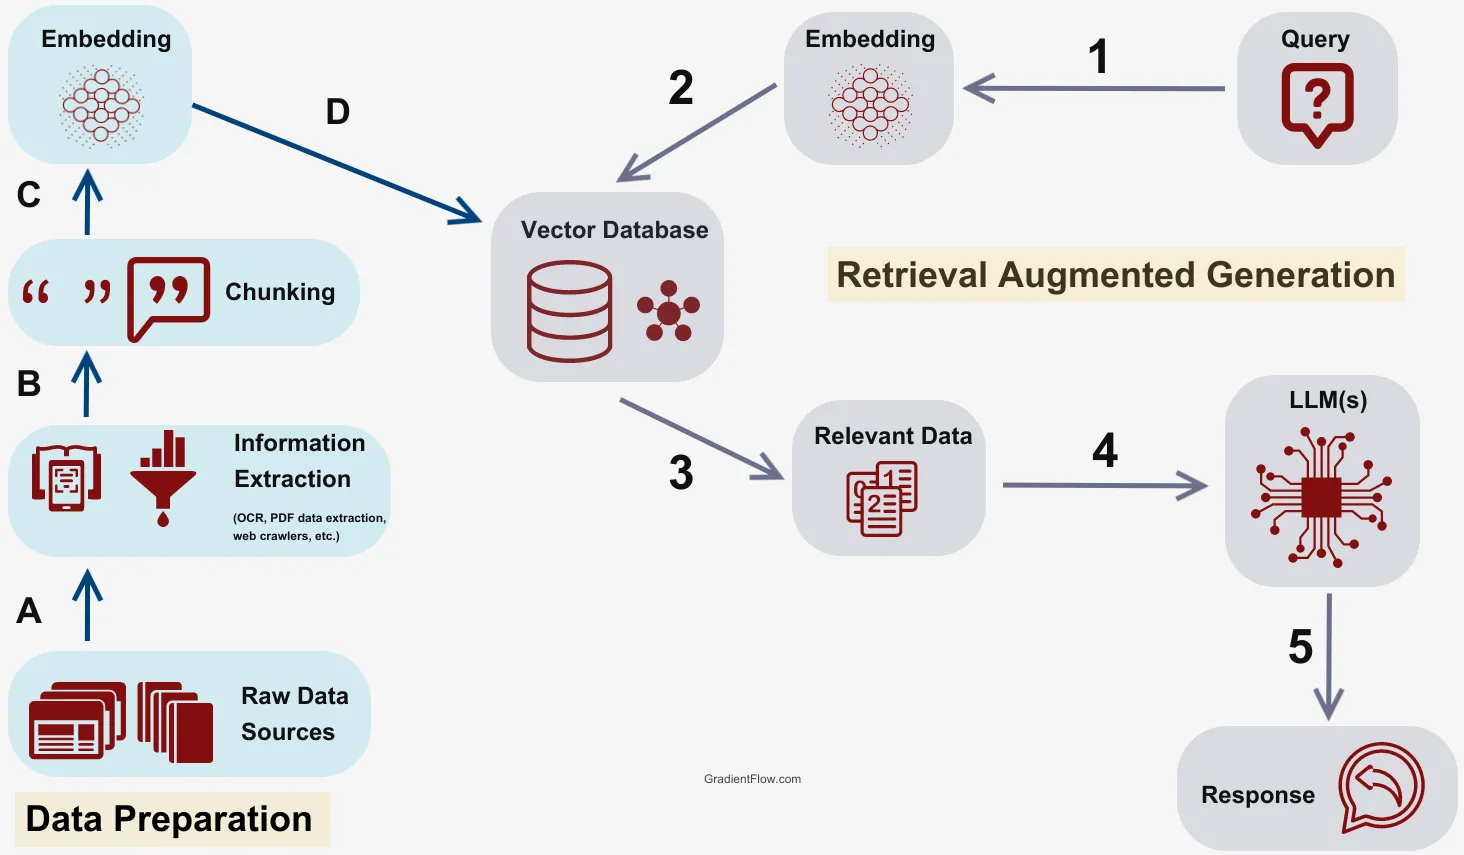
\includegraphics[width=\textwidth]{RAG.png}
		\centering
	\end{figure}
\end{displayquote}
\newpage

RAG kan hier dienst doen als een mogelijke plaatsvervanger voor manuele research en het opstellen van communicatiedocumenten (zoals aangetekende brieven, invorderingen, ...). Deze optie zal in
een later stadium van deze bachelorproef geëvealueerd worden. Advocatuur is een heel toepasselijk gebied voor RAG:

\begin{displayquote}
	\textit{"Practically, RAG is likely preferable in environments like
		legal, customer service, and financial services where the ability to
		dynamically pull vast amounts of up-to-date data enables the most accurate and comprehensive responses."} \autocite{MediumRAG}
\end{displayquote}

\section{Het automatiseren van administratieve taken}
\subsection{Probleemstelling}
Het manueel en persoonlijk afhandelen van 'simpele' administratieve taken door een advocaat zelf kan heel veel tijdverlies veroorzaken.
Een digitale assistent kan bepaalde zaken overnemen, zoals het inplannen van consultaties, agendabeheer en routinecommunicatie. \\
In hoeverre kan een systeem dit overnemen? Is dit mogelijk?

De eerste zaak waar een programmeur zijn hoofd over kan breken:
hoe kunnen we een assistent toegang (lezen en schrijven) geven tot de persoonlijke agenda's van advocaten, programma's en persoonlijke omgevingen?

Wat als er iets fout gaat en heel de agenda wordt overschreven met nutteloze data?
Wat als afspraken bevestigd worden maar niet ingepland?

Het is ook niet echt ethisch verantwoord als een cliënt een som betaalt voor persoonlijke aandacht en communicatie en dan gegenereerde content voorgeschoteld krijgt.
Aan de andere kant kan het ook zijn dat een advocaat in tijdsnood raakt en dan is het natuurlijk handig dat hij een snelle "content boost" ter zijn beschikking heeft.

\subsection{Mogelijke hulpmiddelen en oplossingen}
Een LLM (dat ook gebruikt kan worden bij voorgaande zaken) is hiervoor een ideale oplossing.
Het kan dienen ter inspiratie of ter generatie van een volledig document.
Natuurlijk moet een advocaat een persoonlijke behandeling verstrekken aan de cliënt dus deze optie wordt best alleen gebruikt in geval van nood.

Aan de andere kant kan een virtuele assistent wel instaan voor taken zoals agenda- en memobeheer.
Een dergelijke implementatie vereist integratie met bestaande software zoals Office365 (Microsoft) en ERP programma's.
Ook de analyse van persoonlijke communicatie van een advocaat en zijn cliënt zal ingebracht moeten worden in trainingsdata,
wat ons naadloos overbrengt naar de veiligheid van data tijdens het gebruik en training van digitale tools en assistenten.

\section{Privacy en veiligheid  van data}
In advocatenkantoren wordt op een dagelijkse basis omgegaan met vertrouwelijke informatie van cliënten.
Het is dan natuurlijk meer dan logisch dat de veiligheid van dergelijke informatie van elementair belang is.
Een citaat van "Legal buddies" staaft een paar protocollen om datasecurity en compliance in acht te nemen. 
Dit om met strikte dataregulaties zoals GDPR in de Europese Unie te volgen:

\begin{displayquote}
	\textit{"Proper protocols must be implemented to keep sensitive case data protected and align usage to regional regulations.}
	\begin{itemize}
		\item \emph{ When working with legal AI systems, law firms must implement security controls like data encryption, access management, network segmentation, and intrusion detection.}
		\item \emph{ Usage and data sharing policies should conform to relevant privacy laws and professional ethics rules around legal data confidentiality.}
		\item \emph{ Firms can request third-party audits of AI provider security infrastructure for assurance on protection mechanisms.}
		\item \emph{ Using on-premise AI options instead of cloud-based ones may better align with internal compliance rules and risk tolerance levels.}
		\item \emph{ Regional laws may also dictate data residency and cross-border transfer restrictions. Understanding jurisdictional nuances allows appropriate legal AI adoption.}
		\item \emph{ Overall, prudent security and compliance positioning is vital for law firms exploring innovative technologies like AI-powered legal assistants. Partnering with trusted, vetted providers also reduces risk exposure.}
	\end{itemize}

	\textit{With deliberate planning around privacy, ethics and regional legislation, firms can safely pursue AI efficiency gains."}\autocite{LegalBuddies}
\end{displayquote}

Bij verdere research blijkt het grootste risico dat data van cliënten (onveilig) over het internet gestuurd wordt of dat de data blijft plakken op de cloud server van een externe tool.
De betere en veiligste optie blijkt hier om oftewel lokaal of in private cloud te hosten. 
\\In het hoofdstuk "Methodologie" zullen verschillende technologieën besproken worden om een dergelijke setup te bereiken.

\section{Gebruiksgemak en aanpassing}
Een van de belangrijkste dingen in het inbrengen van nieuwe software in een bestaand kantoor is het gebruiksgemak en toegankelijkheid van de nieuwe programma's. 
Om deze zaken te garanderen, moeten er een paar principes nauwlettend gevolgd worden. 
De beste manier om een design te krijgen waar de gebruiker centraal in staat is het verstaan van de requirements, pijnpunten en workflows van advocaten. 
Dit is van elementair belang om een intuïtief systeem te bouwen dat naadloos integreert in hun workflow. Natuurlijk is dit niet het enige.
Laten we samen een paar belangrijke aspecten overlopen.

\subsection{Een intuïtieve interface}
De interface van een digitale assistent moet er overzichtelijk en netjes uitzien. 
Makkelijke navigatie is van elementair belang.
Advocaten moeten snel en makkelijk de features kunnen aanspreken zonder al te veel clutter en nutteloze toepassingen. 
De beste interface is er een die minimaal en ontworpen is met de gebruiker in het achterhoofd. 
Deze stelling kan onderbouwd worden met enkele designprincipes uit een artikel van Zefort.com:

\begin{displayquote}
	\textbf{Simplicity and clarity:}
	\textit{By reducing complexity and providing clear instructions, legal services become more user-friendly and facilitate better access to justice for all.}
	\autocite{Zefort}

	\textbf{Visual Hierarchy and Information Organization:}
	\textit{Prioritizing content through size, color, and contrast also aids in emphasizing key points and important details.}
	\autocite{Zefort}

	\textbf{Clear and Accessible Navigation:}
	\textit{A well-designed navigation system helps lawyers, clients, and other users locate the information they need with minimal effort.}
	\autocite{Zefort}
\end{displayquote}

\subsection{Natural language processing}
Om de leercurve van een digitale assistent te verlagen, moet deze in staat zijn om queries in natuurlijke taal te kunnen verwerken.
Dit laat advocaten en medewerkers toe om de assistent te benaderen op dezelfde manier als een menselijke collega. Meer over NLP in het hoofdstuk methodologie.

\subsection{Naadloze integratie}
Een dichte integratie met de bestaande software die gebruikt wordt is misschien wel één van de belangrijkste van de drie. Het succes van deze implementatie valt of staat met hoe makkelijk
een advocaat ze kan integreren in hun bestaande workflow. Dit elimineert manuele invoer van manuele data of het constant switchen tussen verschillende applicaties.

In conclusie: het succes van een digitale assistent (of in extensie bijna iedere digitale toepassing) hangt grotendeels af van de gebruikerservaring.
Als je de voorgaande drie zaken zult prioriteren in de ontwikkeling van een tool, kun je makkelijker het volledige potentieel ervan bereiken en zodoende een kwalitatieve, nuttige tool leveren.

\section{Technology Acceptance Model}
Een van de moeilijke dingen aan het implementeren van nieuwe software is controleren of het wel echt voordeel heeft op de workflow en of de mensen die ermee werken het accepteren. 
Daar heeft Fred Davis in '89 al een oplossing voor gevonden, namelijk het Technology Acceptance Model. 
Dit model focust op de bruikbaarheid en het gebruiksgemak van de applicaties via een paar componenten:

\begin{itemize}
	\item \textbf{Perceived Usefulness:} De graad in hoeverre een persoon gelooft dat een bepaald systeem hun productiviteit zal boosten
	\item \textbf{Perceived Ease of Use:} De graad in hoeverre een persoon gelooft dat een bepaald systeem makkelijk te gebruiken valt
	\item \textbf{Attitude towards Using:} De algemene attitude van een persoon tegenover het gebruik van een bepaald systeem, beïnvloed door bovenstaande
	\item \textbf{Behavioral Intention to Use:} De sterkte van de intentie van de gebruiker om een bepaald systeem te gebruiken
	\item \textbf{Actual System Use:} Het werkelijke gebruik van een bepaald systeem
\end{itemize}

Merk op dat deze componenten geobserveerd worden over verschillende tijdsperiodes. De laatste zal maar geobserveerd kunnen worden na de effectieve implementatie. 

